!TEX root = main.tex
\renewcommand{\labelenumi}{\alph{enumi})}

\section*{Examen 1}

\begin{questions}
\question \textbf{1.5pts.} Obtener una gramática regular que genere el mismo lenguaje que el aceptado por el
siguiente autómata (muestra el proceso):

\begin{center}
    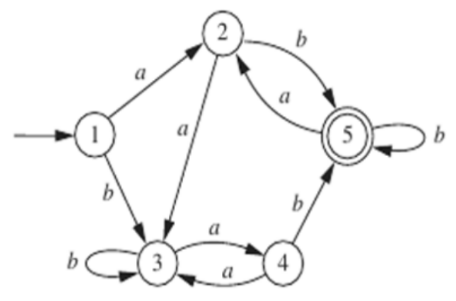
\includegraphics[scale=0.40]{exam4/e4fa.png}
\end{center}

    El lenguaje que genera las cadenas es:

    $L = (a + b)^{+}(a + b)^{*}b^{+}$

    La gramatica regular que genera las cadenas es: 

    $G = <V,T,S,P>$

    $V = \{D\}$

    $T = \{S, A, B, C\}$

    Reglas de produccion P:

    $S \rightarrow \{aA | bB\}$

    $A \rightarrow \{aB | bD \}$

    $B \rightarrow \{aC | bB\}$
    
    $C \rightarrow \{aB | bD\}$

    $D \rightarrow \{aA | bD | \epsilon \}$
    

\question \textbf{1.5 pts.} Genera un autómata finito cuyo lenguaje de aceptación es el mismo que el generado por
la siguiente gramática:

$S \rightarrow \{aA | \epsilon \}$  $D \rightarrow \{bC | b | aF | a \}$

$A \rightarrow \{aB | bE \}$  $E \rightarrow \{bE | aF | a | \epsilon \}$

$B \rightarrow \{aA | bC | b \}$  $F \rightarrow \{aF | a | bF | b \}$

$C \rightarrow \{bD | aF | a | bS\}$ 

        
\begin{center}    
    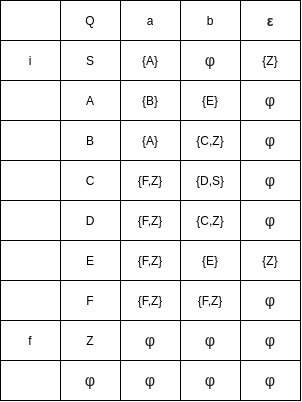
\includegraphics[scale=0.40]{exam4/e4t1.png}
    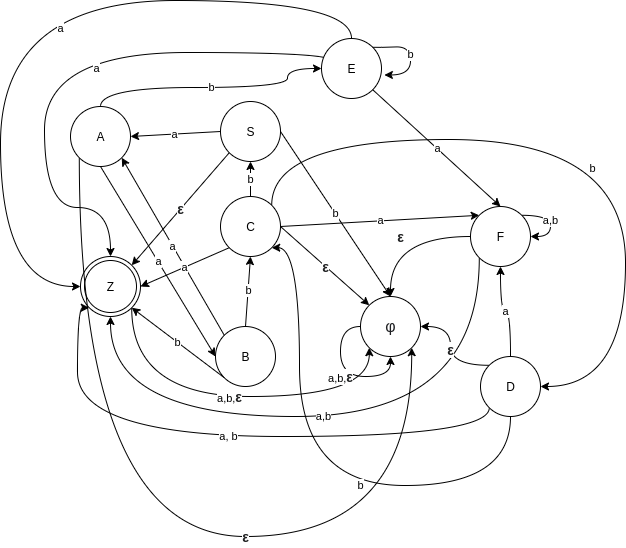
\includegraphics[scale=0.40]{exam4/e4a4.png}
\end{center}
 


\question La gram\'atica G permite construir el siguiente \'arbol de 
derivaci\'on para la cadena abccc


\begin{center}
    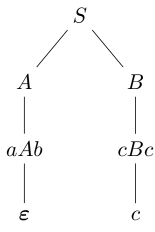
\includegraphics[scale=0.40]{exam4/e4a1.png}
\end{center}


\begin{enumerate}
    a) (1 pt.) Dar la definición formal de G, asumiendo que las variables, terminales y producciones de G son únicamente las
    involucradas en el árbol anterior.

    \begin{solution}

        $<V,T,S,P>$

        V = \{S,A,B\}
        T = \{a,b,c\} \\
        S es el s\'imbolo inicial. \\
        P Son las reglas de producci\'on: \\
        $S \rightarrow A | B$ \\
        $A \rightarrow aAb | \epsilon$ \\
        $B \rightarrow cBc | c$ \\
    \end{solution}

    b) (1 pt.) Construya dos derivaciones para abccc cuyo árbol de derivación sea el anterior y de manera que una sea por la
    izquierda y la otra arbitraria.

    \begin{solution}

        Por la izquierda: 
        1. $S \rightarrow AB \rightarrow aAbB \rightarrow a \epsilon bB
        \rightarrow abB \rightarrow abcBc \rightarrow abccc$

        Arbitraria:
        2. $S \rightarrow AB \rightarrow AcBc \rightarrow Accc
        \rightarrow aAbccc \rightarrow a\epsilon bccc \rightarrow abccc$
    \end{solution}

    c) (1.5 pts.)¿Quién es L(G)? justifique su respuesta.

    \begin{solution}
        $L(G) = \{a^{n}b^{n}c^{m} | n \geq 0, m \geq 3 | \text{m es impar}\}$
        \\
        \text{n es mayor o igual que cero para denotar que ab pueden estar o no, y m igual a 3 ya que tiene que haber minimo 3 c}
    \end{solution}


\end{enumerate}

\begin{center}
    4. Considere la siguietne gram\'atica G:

    $S \rightarrow Ab | aaB$

    $A \rightarrow a | Aa$

    $B \rightarrow a | b | c$
\end{center}

\begin{enumerate}
    \item (1 pts.) Demuestre que G es ambigua mostrando dos \'arboles distintos de derivac\'ion \'unico a\'arbol de derivaci\'on para una misma cadena w de su elecci\'on.
    \begin{center}        
        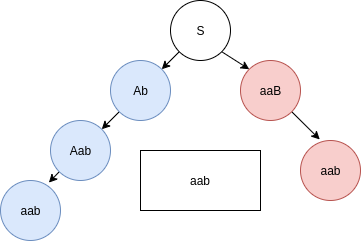
\includegraphics[scale=0.40]{exam4/e4a2.png}

        Como se puede ver marque un camino con rojo y otro con azul para que se vea
        que son arboles diferentes.
    \end{center}
    
    \item (1.5 pts.) Defina una gram\'atica G' no ambigua equivalente a G.
    \begin{center}
        $S \rightarrow Aa | Ab | Ac$

        $A \rightarrow a | Aa$
    \end{center}
    \item (1 pts.) Muestre el \'unico a\'arbol de derivaci\'on para la cadena w empleada ene l inciso a).
    \begin{center}        
        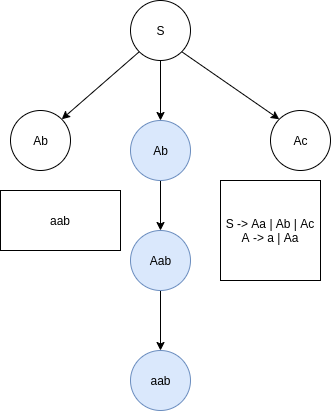
\includegraphics[scale=0.40]{exam4/e4a3.png}
    \end{center}
\end{enumerate}



